% --------- document setup ---------
\documentclass[12pt]{article}
\usepackage[
    left=1in,
    right=1in,
    top=0.5in,
    bottom=0.5in,
    includehead,
    includefoot
]{geometry}
\setlength{\parskip}{0.75em} % larger jumps at end of paragraph
\setlength{\parindent}{0pt} % no indent
\pagenumbering{gobble} % no page numbers

% --------- packages ---------
\usepackage{graphicx} % required for inserting images
\usepackage{multicol} % two column feature
\usepackage{hyperref} % hyperlinks
\usepackage{etoolbox} % if-then-else logic
\usepackage{amsmath, amsfonts, amssymb, amsthm, mathrsfs} % math
\usepackage{float} % figure env
\usepackage{tikz} % drawing things
\usetikzlibrary{automata, positioning}
\usepackage{xcolor} % colors
\usepackage[most]{tcolorbox} % answer boxes
\usepackage{fancyhdr} % header
\usepackage{fancyvrb} % fancy verbatim
\usepackage{ifthen} % conditional statements
\usepackage{lipsum} % filler text
\usepackage{xstring} % For string manipulation
\usepackage{enumitem} % for hint hanging indent
\usepackage{outlines} % for outlines
\usepackage{fancybox} % for nice title page box
\usepackage{soul} % for strikethrough
\usepackage{algorithm} % for algorithms
\usepackage{dsfont}

\newcommand{\note}[1]{{\footnotesize
        \begin{description}
                [leftmargin=3.4em,style=nextline]
            \item[Note:] {#1}
        \end{description}}
}

% --------- Header + Title ---------
\renewcommand\maketitle{
    \begin{center}
        \shadowbox{\parbox{5.3in}{{\small {\bf {\sc Georgia Tech Spring 2025
                \hfill CS 3511: Honors Algorithms}}}
                \medbreak
                \begin{center}
                    {\large \bfseries \reportTitle}
                \end{center}
                \medbreak
                Authors: {\em \authors}
                \newline
                Date: \reportDate
            \vspace{2pt}}
        }
        \vspace{6pt}
    \end{center}
}

% --------- Custom symbols ---------
\newcommand{\C}{\mathbb{C}}
\newcommand{\E}{\mathbb{E}}
\newcommand{\F}{\mathbb{F}}
\newcommand{\N}{\mathbb{N}}
\renewcommand{\P}{\mathbb{P}}
\newcommand{\Q}{\mathbb{Q}}
\newcommand{\R}{\mathbb{R}}
\newcommand{\Z}{\mathbb{Z}}
\newcommand{\Var}{\operatorname{Var}}
\newcommand{\bigO}{\mathcal{O}}
\newcommand{\Ptime}{\mathrm{P}}
\newcommand{\NPtime}{\mathrm{NP}}
\newcommand{\poly}{\text{poly}}
\newcommand{\Alg}{\mathcal{A}}
\newcommand{\Opt}{\operatorname{OPT}}
\newcommand{\dx}{\ensuremath{\mathrm{d}x}}
\newcommand{\floor}[1]{\left\lfloor #1 \right\rfloor} % for floor
\newcommand{\ceil}[1]{\left\lceil #1 \right\rceil} % for ceiling

% ------------ Document ------------
\begin{document}

\newcommand{\reportTitle}{Final Project}
\newcommand{\reportDate}{Wednesday 4/16/25}

\newcommand{\authors}{Arjun Sheshadri, Vilohith Gokarakonda, Yiqi Sun, Tyler Huang}

\maketitle

\section{Introduction}

Suppose if you have a graph $G = (V, E)$ with a given adjacency matrix, which represents where any two nodes are connected to each other. Suppose you wanted to find the shortest path to one node, using all nodes as a starting point.

Shortest distances between all pairs of nodes in a graph is important for its real world applications in communication networks, social graphs, and more. Edges in such graphs can be added and removed at any time, so being able to efficiently maintain all pairs distances is crucial. Using the Floyd-Warshall Algorithm, we are able to accomplish this in $\bigO(n^3)$ time. However, this becomes inefficient for larger or frequently changing graphs.

This report explores a \textit{dynamic algorithm} described in Jan van den Brand's \href{https://www.dropbox.com/scl/fi/zjfbk8dbxbzcn05dr8l11/fall22_daa_lecturenotes.pdf?rlkey=g6z7z1hvj7jknvlpy1s3dqcjw&e=1&st=13r18doq&dl=0}{notes} for maintaining All-Pairs-Shortest-Paths (\texttt{APSP}) in directed graphs with or without edge weights. Instead of recalculating shortest distances from scratch every update, it efficiently maintains a data structure where all distances can be updated in $\displaystyle \tilde \bigO(n^{2.5})$ time when an edge to a single vertex is added or removed. Specifically, it uses concepts from dynamic algebraic algorithms, involving polynomial matrix inverses to represent path information, and extending them to full distances with random sampling and Dijkstra's algorithm.

In this report, we present the problem statement, and the technical background relevant to the paper, including ring algebra, polynomial matrices, and how edges are updated. We also cover the steps to the solution, and connect this approach to the original groundbreaking \href{https://www.dropbox.com/scl/fi/5w4k0lg0u8e36zugapp6c/Sankowski-COCOON-05-subquadratic-dynamic-distances.pdf?rlkey=5eahwsl7a49kwxyvlr7yqyoz3&e=2&st=d3zo7owc&dl=0}{paper} by Sankowski, which can do updates in $\displaystyle \tilde \bigO(n^{1.932})$  randomized time and queries in $\displaystyle \tilde \bigO(n^{1.288})$ randomized time. Specifically, we compare their mathematical foundations, update operations, applications, and time complexities.

\section{Problem Statement}

Given a graph $G(V, E)$, we want to develop a data structure that can maintain \texttt{APSP} dynamically with an initial overhead $\displaystyle \tilde \bigO(n^{3.5})$ time and supports queries and updates in $\displaystyle \tilde \bigO(n^{2.5})$ time. Since this algorithm is optimized for maintaining \texttt{APSP} for changing graphs (hence requires a dynamic algorithm), having a time complexity of $\displaystyle \tilde \bigO(n^{2.5})$ is more efficient compared to the naive approach which takes $\bigO(n^3)$ time for queries and updates.

\newpage

Specifically, we will be working towards proving the following theorem:

\textbf{Theorem 1.0.0}: \emph{There exists a data structure that supports the following operations}:
\begin{enumerate}
    \item \textsc{Initialize($G = (V, E)$)} \emph{Initialize an $n$-node graph and return \texttt{APSP} in $\displaystyle \tilde \bigO(n^{3.5})$ time.}
    \item \textsc{Update($v,\,E^+,\,E^-$)} \emph{Given a vertex $v$ and two sets of edges $E^+\subseteq(\{v\}\times V\cup V\times\{v\})$ to insert and $E^-$ to delete (all incident to $v$), update $G$ and return the new \texttt{APSP} in $\displaystyle \tilde \bigO(n^{2.5})$ time.}
\end{enumerate}

Additionally, we will be extending this theorem using Sankowski's paper:

\textbf{Theorem 1.0.1}: \emph{There exists a data structure that supports the following operations}:
\begin{enumerate}
    \item \textsc{Initialize($G = (V, E)$)} \emph{Preprocess in $\displaystyle \tilde \bigO(n^{3})$ time.}
    \item \textsc{Update($e$)} \emph{Insert or delete a single edge $e\in V\times V$ in $\bigO(n^{1.932})$ randomized time.}
    \item \textsc{Query($s, t$)} \emph{Return the current distance $\mathrm{dist}_G(s,t)$ in $\bigO(n^{1.288})$ randomized time.}
\end{enumerate}
\emph{All operations succeed with high probability over the random choices.}

We will be covering general overviews of topics that help toward understanding the intuition behind these theorems in the next section.

\section{Technical Background}

\subsection{Matrix Multiplication Recap and Naive APSP} \label{sec:3.1}

Matrix multiplication is an important concept that we will be making extensive use of to understand the technical components in this report. You are already familiar with the basic method of multiplying two matrices with the same inner dimension, where you multiply the $n$-th row of the first matrix with the $n$-th column of the second matrix. Below is a visual representation:

\[
    \begin{bmatrix}
        a & b \\
        c & d
    \end{bmatrix}
    \begin{bmatrix}
        e & f \\
        g & h
    \end{bmatrix}
    =
    \begin{bmatrix}
        a \cdot e + b \cdot g & a \cdot f + b \cdot h \\
        c \cdot e + d \cdot g & c \cdot f + d \cdot h
    \end{bmatrix}
\]

Notice how in each $(i, j)$ entry of the product matrix, we compute the \emph{dot product} of the vector that forms the $i$-th row of the first matrix and the $j$-th column of the second matrix. The \emph{dot product} is simply an operation on the entries of two vectors involving the typical $+$ and $\times$ operations.

Let's take a quick detour from matrix multiplication to talk about the well-known Floyd-Warshall algorithm for computing \texttt{APSP}. The key realization to understanding this algorithm is that between some start node $s$ and some terminal node $t$, the shortest path from $s \to t$ is the shorter path we can get from directly traveling from $s \to t$ vs. the path we get by traveling from $s$ to some intermediate node $k$ and then from $k$ to $t$. For a visualization, consider the trivial example below:

\begin{center}
    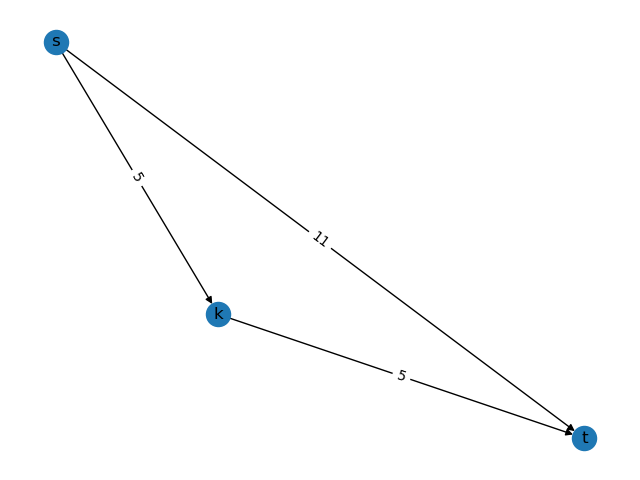
\includegraphics[scale=0.5]{media/Figure_1.png}
\end{center}

In the above graphic, the direct path from $s \to t$ has a cost of 11, while the path from $s \to k$ has a cost of 5 and the path from $k \to t$ has a cost of 5 as well. We can see that if we take $\min \{\mathrm{dist}_{s,t} = 11, \mathrm{dist}_{s,k} + \mathrm{dist}_{k,t} = 10 \}$, we get that by considering the intermediate node $k$, we arrive at a cheaper path from $s$ to $t$.

How does the above logic tie into matrix multiplication? Well, it might be intuitive to think of graphs in terms of adjacency matrices and the core Floyd-Warshall computation as a dot product between some vector $u$ that represents the shortest known paths from the starting node $s$ to all possible intermediate nodes $k$, and another vector $v$ that represents the shortest paths from all possible intermediate nodes $k$ to the terminal node $t$. Let's see an example of this analogy on the simple graph presented earlier:

\begin{quote}
    Consider the adjacency matrix $A$ for the graph presented earlier:

    \[
        A =
        \bordermatrix{
            & s & k & t \cr
            s & 0 & 5 & 11 \cr
            k & \infty & 0 & 5 \cr
            t & \infty & \infty & 0 \cr
        }
    \]

    Notice that in $A$, the $(i, j)$ entry represents the cost of the \emph{direct} path from node $i$ to node $j$. The rows and columns are labeled with their appropriate nodes on the borders.

    For the sake of computation, let's take the row $s$ and the column $t$ of the matrix as our $u$ and $v$ vectors. That is, let

    \[
        u =
        \begin{bmatrix}
            0 & 5 & 11
        \end{bmatrix}
        \qquad
        v =
        \begin{bmatrix}
            11 \\
            5 \\
            0
        \end{bmatrix}
    \]

    Just for clarity, recall that $u$ represents the shortest known path between the starting node $s$ and every other node $k$ in the graph. For column $s$ of $u$, the shortest path cost is 0 since we are already at $s$. For column $k$ of $u$, the path cost is 5 since the edge $s \to k$ on the graph has a cost of 5. For column $t$ of $u$, the path cost is 11 since the edge $s \to t$ has a cost of 11. In general, we see that each \emph{column} in $u$ represents the cost of the edge $s \to \textit{column in u}$. Following a similar logic, notice that in the vector $v$, each \emph{row} represents the cost of the edge $\textit{row in v} \to t$. Both \textit{column in $u$} and \textit{row in $v$} represent all the nodes in the graph.

    Let's replace the numbers in $A$ with symbols, and see what happens when we take the dot product of $u$ and $v$:

    \[
        A =
        \bordermatrix{
            & s & k & t \cr
            s & \mathrm{dist}_{s \to s} & \mathrm{dist}_{s \to k} & \mathrm{dist}_{s \to t} \cr
            k & \mathrm{dist}_{k \to s} & \mathrm{dist}_{k \to k} & \mathrm{dist}_{k \to t} \cr
            t & \mathrm{dist}_{t \to s} & \mathrm{dist}_{t \to k} & \mathrm{dist}_{t \to t} \cr
        }
    \]

    \[
        u =
        \begin{bmatrix}
            \mathrm{dist}_{s \to s} & \mathrm{dist}_{s \to k} & \mathrm{dist}_{s \to t}
        \end{bmatrix}
        \quad
        v =
        \begin{bmatrix}
            \mathrm{dist}_{s \to t} \\
            \mathrm{dist}_{k \to t} \\
            \mathrm{dist}_{t \to t}
        \end{bmatrix}
    \]

    Let's see what happens when we take the dot product of $u$ and $v$, which will be the $(s, t)$ entry of the matrix $A^2$:

    \begin{eqnarray}
        A^2_{(s,t)}
        &= \mathrm{dist}_{s \to s} \times \mathrm{dist}_{s \to t} \\
        &+ \; \mathrm{dist}_{s \to k} \times \mathrm{dist}_{k \to t} \\
        &+ \; \mathrm{dist}_{s \to t} \times \mathrm{dist}_{t \to t}
    \end{eqnarray}

    Based on the dot product formula, it seems that in the $(s, t)$ entry of the matrix $A^2$, we are able to calculate some information involving all paths from node $s$ to node $t$ involving one intermediate step through all the other nodes in the graph. Particularly, the product on line $(1)$ gives us information regarding the path $s \to s \to t$, the product on line $(2)$ gives us information regarding the path $s \to k \to t$, and the product on line $(3)$ gives us information regarding the path $s \to t \to t$. You may notice the paths $s \to s \to t$ and $s \to t \to t$ are simply the same as the path $s \to t$, a direct path from $s$ to $t$ with no intermediate nodes. It may become apparent to you that by induction, the matrix $A^3_{(s, t)}$ stores the shortest path between $s \to t$, $s \to k \to t$ for all graph vertices $k$, and $s \to k_0 \to k_1 \to t$ for all combinations of nodes $k_0$ and $k_1$ in the graph. We can say that the adjacency matrix $A^n_{(s, t)}$ stores the shortest path from $s$ to $t$ using \emph{up to} $n$ intermediate vertices.

    {\footnotesize Why is the induction apparent? If we multiply adjacency matrix $A^n$ by adjacency matrix $A^m$, we notice that we will be considering paths of the form $s \to k_0 \to \cdots \to k_{n - 1} \to k_{n} \to k_{n + 1} \to \cdots k_{n + m - 1} \to t$. The total length of this path is $n + m$, which is also the power of the product as $A^n \times A^m = A^{n + m}$, and the number of intermediate nodes is $n + m - 1$.}
\end{quote}

As shown in the above analogy, we are essentially able to store the result of a dot product operation between the path lengths of $s \to t$ and $s \to k \to t$ for every intermediate node $k$ in the graph. As we explained earlier during our discussion of Floyd-Warshall's algorithm, we specifically need to compute the minimum cost path between all the aforementioned products from the dot product calculation. In the next section, we will show how we can override the standard $+$ and $\times$ operations such that simply computing the squares of adjacency matrices allows us to solve \texttt{APSP}, and we will also explain how other properties of environments with overridden $+$ and $\times$ operations may help us solve \texttt{APSP} more efficiently.

\subsection{Abstract Algebra Overview and Ring Operations} \label{sec:3.2}

In this section, we cover the basics of the field of abstract algebra as relevant in solving the \texttt{APSP} problem. As we showed in section~\ref{sec:3.1}, on an adjacency matrix of power $A^n$, the $(s, t)$ entry encodes information regarding the dot product between $s$-$t$ paths involving up to $n$ intermediate nodes. When we explained our theory regarding Floyd-Warshall's algorithm, we mentioned that we somehow need to store the minimum cost path between all of the path costs ($s \to t, s \to k_0 \to t, \ldots, s \to k_0 \to k_1 \to \cdots \to k_{n - 1} \to t$) that make up the individual products in the dot product. We may now ask ourselves, when computing a dot product in the form:
\[
    \begin{split}
        A^2_{(s,t)}
        &= \mathrm{dist}_{s \to s} \times \mathrm{dist}_{s \to t} \\
        &+ \; \mathrm{dist}_{s \to k} \times \mathrm{dist}_{k \to t} \\
        &+ \; \mathrm{dist}_{s \to t} \times \mathrm{dist}_{t \to t}
    \end{split}
\]
Is it possible to override the $+$ and $\times$ operations in order to suit our desired $\min$ and $+$ operations?

It turns out this is entirely possible as long as our overridden $+$ and $\times$ operations adhere to the rules of \emph{algebraic rings}. A ring is an algebraic structure—that is, a set of elements together with two binary operations $\oplus$ and $\otimes$—that satisfies certain axioms:

\begin{quote}
    $S$ is an algebraic \emph{semiring} defined as $(S, \oplus, \otimes)$. The below conditions must be met:

    \begin{enumerate}
        \item $(S, \oplus)$ is an abelian group. In other words, it satisfies the commutative property that $\forall a, b \in S : a \oplus b = b \oplus a$ and it satisfies the identity that $\forall a \in S : a \oplus 0_S = a$, where $0_S$ refers to the zero element in $S$.
        \item $(S, \otimes)$ is a monoid. In other words, it satisfies the identity $\forall a \in S : a \otimes I = a$, where $I$ refers to the identity element, which can typically be thought of as 1.
        \item The $\otimes$ operation must distribute over the $\oplus$ operation. In other words, $\forall a, b, c \in S : a \otimes (b \oplus c) = a \otimes b \oplus a \otimes c$.
        \item $0_S$ is an annihilator in $\otimes$. In other words, $\forall a \in S : a \otimes 0_S = 0_S \otimes a = 0_S$.
    \end{enumerate}

    Alternatively, we define $F$ as an algebraic \emph{field}, denoted as $(F, \oplus, \otimes)$ if it meets the below conditions:

    \begin{enumerate}
        \item $(F, \oplus)$ is an abelian group.
        \item $(F \backslash \{0\}, \otimes)$ is also an abelian group, which implies the existence of a multiplicative inverse for every non-zero element.
    \end{enumerate}

    {\footnotesize Note, the difference between a \emph{ring} and a \emph{semiring} is that a semiring does not need to support the additive inverse. Meaning, there does not necessarily have to be a ``negative'' corresponding to each element. Additionally, note that $\otimes$ does not have to be commutative.}
\end{quote}

So how does this tie into our \texttt{APSP} problem?

We can define our dot product over the semiring $(S, \oplus, \otimes)$ where:
\[
    \begin{split}
        & a, b \in \mathds{R} \\
        & a \oplus b = \min\{a, b\} \\
        & a \otimes b = a + b \qquad \text{{\footnotesize Where + is the typical addition}}
    \end{split}
\]
It is straightforward why we can do this, since $(S, \min, +)$ satisfies all of the axioms. You can convince yourself of this fact. It is important to note that $S$ does not have an additive inverse since there is no possible $a, b \in S : \min\{a, b\} = \infty$ unless $a = \infty$ and $b = \infty$.

Now, notice how the dot product defined at the end of section~\ref{sec:3.1} changes. Under our ring $S$, we get:
\[
    \begin{split}
        A^2_{(s,t)}
        &= \mathrm{dist}_{s \to s} \otimes \mathrm{dist}_{s \to t} \\
        &\oplus \; \mathrm{dist}_{s \to k} \otimes \mathrm{dist}_{k \to t} \\
        &\oplus \; \mathrm{dist}_{s \to t} \otimes \mathrm{dist}_{t \to t}
    \end{split}
    \qquad = \qquad
    \min\!\left\{
        \begin{aligned}
            &\mathrm{dist}_{s\to s} + \mathrm{dist}_{s\to t},\\
            &\mathrm{dist}_{s\to k} + \mathrm{dist}_{k\to t},\\
            &\mathrm{dist}_{s\to t} + \mathrm{dist}_{t\to t}
        \end{aligned}
    \right\}
\]
This exactly what we wanted to compute when we discussed Floyd Warshall's algorithm! As you can see, using algebraic rings, we have come up with a system where simple repeated squaring of the adjacency matrix $A$ over the ring $R$ effectively solves \texttt{APSP}. We notice that after squaring the adjacency matrix $n - 1$ times, the result contains the answer to \texttt{APSP}. Since matrix multiplication takes on the order of $\bigO(v^3)$ time, where $v$ is the number of vertices in the graph, and since we must effectively square the adjacency matrix $v$ times, we can see how a min-plus squaring algorithm attains a time complexity of $\bigO(v^4)$ (using naive matrix multiplication).

Our repeated squaring approach can take as little as $\bigO(n^3 \log(n))$ time if we are more efficient in how we implement \emph{binary exponentiation} rather than using naive matrix multiplication for exponentiation. However, the repeated squaring method is still more inefficient than Floyd-Warshall's algorithm, which takes only $\bigO(n^3)$ time. It turns out that both the min-plus repeated squaring approach and Floyd-Warshall's algorithm are performing the same operations to compute \texttt{APSP}, however Floyd-Warshall's algorithm attains more efficiency using \emph{dynamic programming} and ``simulating'' the min-plus matrix multiplications in place. This min-plus repeated squaring approach also lies at the heart of the algorithm mentioned in Jan van den Brand's paper, but before we can conceptualize it, we are going to use our knowledge or algebraic rings to talk about polynomial matrices.

\subsection{Polynomial Matrices} \label{sec:3.3}

Now, let's really start building the foundation to Jan van den Brand's \texttt{APSP} algorithm by taking about adjacency matrices with polynomial entries!

\subsubsection{Unweighted Adjacency Matrices}

First let's build some intuition for why we might want to build polynomial adjacency matrices. Going forward, we are specifically going to talk about \emph{unweighted} adjacency matrices where $A_{(s, t)} = 1$ if there is a directed edge $s \to t$ and $0$ otherwise. When we refer to simple unweighted adjacency matrices, it turns out we can use simple powers of $A$ (ie. $A, A^2, A^3, \ldots, A^n$) and the traditional operations $+$ and $\times$ to achieve a similar effect to our min-plus repeated squaring algorithm that we explained in section~\ref{sec:3.2}. However, instead of tracking in the $A^n_{(s, t)}$ the shortest path between start node $s$ and terminal node $t$ using up to $n$ intermediate nodes, in the $A^n_{(s, t)}$ position, we are instead tracking the \emph{number} of paths that \emph{exist} between $s$ and $t$ on \emph{exactly} $n$ nodes. Why exactly is this? Let's consider a simple example with the graph below:

\begin{center}
    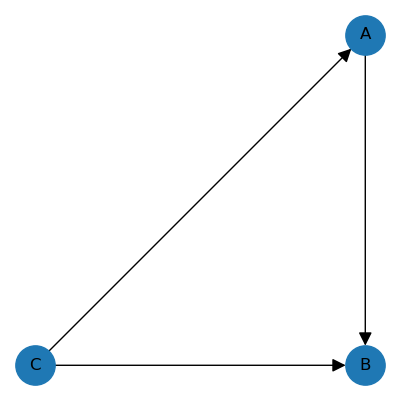
\includegraphics[scale=0.5]{media/Figure_2.png}
\end{center}

\begin{quote}
    We can build the unweighted adjacency matrix for the above graph:

    \[
        A =
        \bordermatrix{
            & A & B & C \cr
            A & 0 & 1 & 0 \cr
            B & 0 & 0 & 0 \cr
            C & 1 & 1 & 0 \cr
        }
    \]

    Notice again how this first degree adjacency matrix only tells us if a \emph{direct} edge exists between any start node and terminal node. Now, pay attention to the following calculations we will perform on two different paths for the sake of example: $C \to B$ and $B \to C$.

    First, let's take $C \to B$. From the graph picture, we can see that there are two paths from $C \to B$. There is one direct path from $C$ to $B$, which is why $A_{(C, B)} = 1$. Additionally, there is another path through intermediate node $A$, which corresponds to the path $C \to A \to B$. Let's see what happens when we calculate $A^2_{(C, B)}$, involving the dot product between the vector formed by row $C$ and the vector formed by column $B$.

    \[
        u =
        \begin{bmatrix}
            1 & 1 & 0
        \end{bmatrix}
        \quad
        v =
        \begin{bmatrix}
            1 \\
            0 \\
            1
        \end{bmatrix}
    \]

    Like we mentioned earlier in section~\ref{sec:3.1}, in this format, $u$ represents the existence of a direct path that begins at node $C$ and ends at every other node in the graph, while $v$ represents the existence of a direct path that begins at every other node in the graph and ends at node $B$. We can think of each product in this dot product as if asking the question ``Is there a \emph{direct} path from $C$ to some node $k$ and then is there a \emph{direct} path from that node $k$ to $B$?'' If the answer is yes to both parts of that question, this individual product amounts to 1. Below is the dot product calculation.

    \[
        u \cdot v = (1 \cdot 1) + (1 \cdot 0) + (0 \cdot 1) = 1
    \]

    You can see how the dot product considers every possible choice of intermediate node, and the result of the dot product should be the number of paths from $C$ to $B$ using exactly one intermediate node. Below is the completed product matrix $A^2$.

    \[
        A^2 =
        \bordermatrix{
            & A^2 & B^2 & C^2 \cr
            A^2 & 0 & 0 & 0 \cr
            B^2 & 0 & 0 & 0 \cr
            C^2 & 0 & 1 & 0 \cr
        }
    \]

    As you can see, if a path starting from $s$ and ending at $t$ exists with exactly one intermediate node, then that position will have a 1 in the matrix. By the same inductive reasoning we used in section~\ref{sec:3.1}, for an adjacency matrix of power $A^n$, the $A^n_{(s, t)}$ entry will track the number of paths from $s$ to $t$ on exactly $n - 1$ intermediate nodes.

    % Now, let's take $B \to C$. There exists no \emph{direct} path in our directed graph from $B \to C$, so we notice that the entry $A_{(B, C)} = 0$. When we square $A$, the entry $A^2_{B, C}$ should contain a 1 if there is a possible path $B \to k \to C$ that takes one intermediate vertex. However, notice that there are no possible paths starting at $B$ and ending at $C$, so we expect $A^2_{(B, C)} = 0$. To calculate this entry, we take the dot product of the vector formed by row $B$ and the vector formed by column $C$.

    % \[
    %     u =
    %     \begin{bmatrix}
    %         0 & 0 & 0
    %     \end{bmatrix}
    %     \quad
    %     v =
    %     \begin{bmatrix}
    %         0 \\
    %         0 \\
    %         0
    %     \end{bmatrix}
    % \]

    % Here, $u$ represents the existence of paths starting at $B$ and ending at any other node in the graph, and $v$ represents the existence of paths starting from any other node in the graph and ending at $C$. Since it is obvious from the graph picture that $B$ has an out-degree of 0 and $C$ has an in-degree of 0, vectors $u$ and $v$ are unremarkably 0 vectors. Therefore, their dot product is also 0 and we find that $A^2_{(B, C)} = 0$.

    It might be self-explanatory why paths that cannot be formed with any number of intermediate nodes, for example $B \to C$ will have $A^n_{(B, C)} = 0 \quad \forall n \in \mathds{Z}^+$.
\end{quote}

\subsubsection{Matix Series Identity}

Let's try something new now. What happens if we want to form the accumulated adjacency matrix $A^{\prime}$ where $A^{\prime}_{(s, t)}$ tracks the total number of $s$-$t$ paths that can take any number of intermediate nodes? A straightforward thing to do would be to consider the sum of matrices of powers counting from 0 to $h$, since each power represents the number of $s$-$t$ paths on exactly $power - 1$ intermediate nodes.

\[
    A^{\prime} = A^0 + A^1 + A^2 + A^3 + \cdots
\]

Does this look familiar to you? You might notice that this sum has a similar format to the infinite geometric series. Note that $A^0 = I$, and the identity matrix adds 1's along the diagonal, which simply adds circular edges from each node to itself. This does not impact any calculations.

We know that a formal geometric series of the form $1 + x + x^2 + \cdots$ can be represented by the generating function

\[
    \frac{1}{1 - x} = 1 + x + x^2 + \cdots
\]

Interestingly, under the conditions of adjacency matrices representing directed acyclic graphs (\texttt{DAG}s), or over a field with random weights, we can use a ``generating function'' to efficiently compute $A^{\prime}$ as well! In particular, we can use the below identity:

\[
    (I - A)^{-1} = A^0 + A^1 + A^2 + A^3 + \cdots
\]

Now, by computing the matrix $A^{\prime} = (I - A)^{-1}$, we have a new matrix we can use to check the existence of an $s$-$t$ path. The $A^{\prime}_{(s, t)}$ entry will be non-zero if a path exists from $s$ to $t$ on any number of intermediate nodes, or $0$ if otherwise. To understand this identity rigorously, we can recall our abstract algebra concepts from section~\ref{sec:3.2}. Notably, our identity only works for \texttt{DAG}s and field matrices since we need a genuine multiplicative inverse to be defined. In a field, every nonzero scalar has an inverse, and determinants live there, so you can talk about $\det(I - A)\neq 0$ and hence $(I - A)^{-1}$ exists.  In an arbitrary ring (say \(\mathbb Z\) or a semiring), you can't guarantee that. Additionally, we need the series $A^0 + A^1 + A^2 + A^3 + \cdots$ to eventually stop since an infinite sum of matrices does not have much meaning unless the tail vanishes. On a \texttt{DAG}, we know the adjacency matrix $A^n = 0$ since there are no paths of length greater than or equal to $n$, as the longest path is of length $n - 1$. However, we will be covering how we can adapt some of these restrictions to general commutative rings so that our algorithm can cover a broader range of matrices.

\subsubsection{Polynomial Matrices as the Next Intuitive Step} \label{sec:3.3.3}

So where do polynomial matrices come into the picture? As discussed previously, our accumulated adjacency matrix $A^{\prime}$ can track the number of $s$-$t$ paths on any number of intermediate nodes. However, just the total number of $s$-$t$ paths does not help us solve \texttt{APSP} since we need some mechanism to determine the \emph{shortest} $s$-$t$ path. An intelligent mechanism to do just this would be to make use of \emph{indeterminates} where we can collect the number of $s$-$t$ paths taking $n$ intermediate nodes as the coefficient of the $x^n$ term of a polynomial.

Let's formalize this theory. Instead of the geometric series we saw earlier, we can instead represent $A^{\prime}$ using a formal power series; we'll call this new matrix $A^{\prime \prime}$:

\[
    A^{\prime \prime} = A^0 x^0 + A^1 x^1 + \cdots + A^n x^n
\]

We can use a similar identity to the one we came up with for $A^{\prime}$ to represent $A^{\prime \prime}$.

\[
    A^{\prime \prime} = (I - xA)^{-1}
\]

We will show why this identity works in subsection~\ref{sec:3.3.4}, but for now, let's see a simple example taking it for granted.

\begin{quote}
    Consider the following graph:

    \begin{center}
        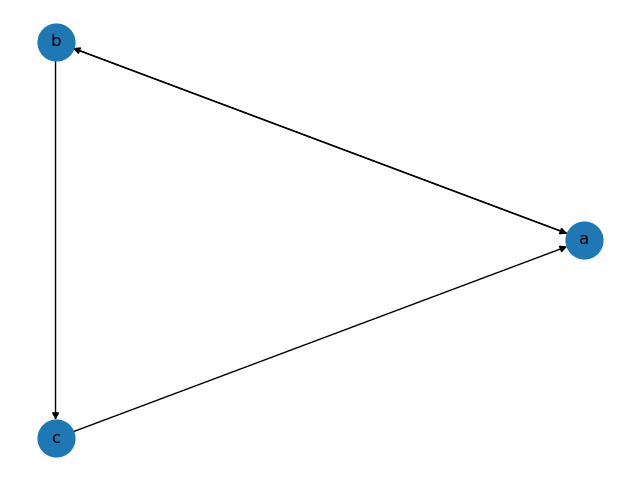
\includegraphics[scale=0.5]{media/Figure_3.png}
    \end{center}

    With the adjacency matrix below:

    \[
        A =
        \bordermatrix{
            & a & b & c \cr
            a & 0 & 1 & 0 \cr
            b & 1 & 0 & 1 \cr
            c & 1 & 0 & 0 \cr
        }
    \]

    We compute $A^{\prime \prime}$ as $(I - xA)^{-1}$:

    \[
        A^{\prime \prime} =
        \left(
            \begin{bmatrix}
                1 & 0 & 0 \\
                0 & 1 & 0 \\
                0 & 0 & 1
            \end{bmatrix}
            -
            x
            \begin{bmatrix}
                0 & 1 & 0 \\
                1 & 0 & 1 \\
                1 & 0 & 0
            \end{bmatrix}
        \right)^{-1}
        =
        \left(
            \begin{bmatrix}
                1 & -x & 0 \\
                -x & 1 & -x \\
                -x & 0 & 1
            \end{bmatrix}
        \right)^{-1}
    \]

    $A^{\prime \prime}$ can be simplified to:

    \[
        A^{\prime \prime} =
        \begin{bmatrix}
            x^2 + 1 & x & x^2 \\
            x^2 + x & x^2 + 1 & x \\
            x & x^2 & 1
        \end{bmatrix}
    \]

    We will cover why the above matrix corresponds to the inverse of $(I - xA)$ in the section~\ref{sec:3.3.4}, but for now, notice how the \emph{coefficient} of the $x^n$ term of each entry $A^{\prime \prime}_{(s, t)}$ indicate the number of $s$-$t$ paths of length $n$. It may occur to you that if we can find an algorithm to efficiently compute $A^{\prime \prime}$ for a given graph, we can solve \texttt{APSP} by simply looking at the lowest degree term of each $A^{\prime \prime}_{(s, t)}$ entry with a non-zero coefficient.
\end{quote}

The example above shows us what we can expect from the matrix $A^{\prime \prime}$, but before we can take the results for granted, we must discuss the details of polynomial matrices make mathematical sense.

\subsubsection{How are Polynomial Matrices Defined?} \label{sec:3.3.4}

Before we get ahead of ourselves, let's understand how exactly we can even define matrices over polynomials and how we can expect them to have inverses. To understand this properly, we will be referring to the abstract algebra concepts we defined in section~\ref{sec:3.2}.

We traditionally think of matrices as algebraic structures that contain numbers, but in reality we just make the assumption that the matrices we encounter are defined over a \emph{ring} $R$ that contains the real numbers. To pass from ``numeric'' matrices to polynomial matrices, we must consider defining matrices over the ring $R[x]$, which replaces each scalar in $R$ with a polynomial in the indeterminate $x$.

Let's be a little more precise in what we mean. For our matrix $A^{\prime \prime}$, we notice that any entry $A^{\prime \prime}_{(s, t)}$ is of the form

\[
    A^{\prime \prime}_{(s, t)} = \alpha_0 x^0 + \alpha_1 x^1 + \cdots
\]

where $\alpha_0, \alpha_1, \ldots$ are \emph{integers} in $\mathds{Z}$. We can specifically define $R[x]$ as a ring that suits this purpose. In particular:

\begin{enumerate}
    \item $R[x]$ is defined over the set of polynomial with integer coefficients, which is represented as $\mathds{Z}[x]$
    \item $(R[x], \oplus)$ is defined as typical polynomial addition where we can combine like terms
    \item $(R[x], \otimes)$ is defined as typical polynomial multiplication, which involves convolving the coefficients of each polynomial
\end{enumerate}

While this definition of $R[x]$ allows us to define polynomial matrices, we still cannot assume that a polynomial matrix has an inverse, which we use in our $A^{\prime \prime}$ identity. Recall earlier where we specifically defined the identity for $A^{\prime}$ to only work over \emph{fields}, where every non-zero scalar was defined to have a multiplicative inverse and we also assumed that we only deal with \texttt{DAG}s to get rid of the infinite matrix sum. While we cannot make the same assumptions for a general commutative ring like $R[x]$, we can show that under the below listed conditions, the matrix $A^{\prime \prime} = (I - xA)^{-1}$ always entries that have a multiplicative inverse and are finite series.

\begin{enumerate}
    \item To make sure that all the entries of $A^{\prime \prime}$ are finite, we can define all polynomial arithmetic to consider only polynomial modulo $x^h$. Specifically, we will redefine $R[x]$ as $\mathds{Z}[x] / \langle x^h \rangle$. When we talk about a polynomial modulo $x^h$, we simply mean that we truncate all of the polynomial terms that have a degree greater than $h$.

        {\footnotesize A size effect of considering only $\mathds{Z}[x] / \langle x^h \rangle$ is that we won't be able use $A^{\prime \prime}$ to track paths of length greater than $h$. We will discuss this more in section~\ref{sec:3.5} and section~\ref{sec:4}}

    \item In the ring $R[x] = \mathds{Z}[x] / \langle x^h \rangle$, the polynomial $p(x)$ is a unit (i.e. invertible) if and only if its constant term is a unit in $\mathds{Z}$. In other words,

        \[
            p(x) = \alpha_0 x^0 + \alpha_1 x^1 + \cdots + \alpha_{h - 1} x^{h - 1}
        \]

        and we notice that there cannot be a $q(x)$ such that $p(x) \cdot q(x) \equiv 1 \mod x^h$ if $\alpha_0$ is not invertible in $\mathds{Z}$. Since we defined $(A^{\prime \prime})^{-1} = (I - xA)$, entries along the diagonal of $(I - xA)$ must have a non-zero constant term. We may notice in this matrix that the identity matrix guarantees constant terms of 1 along the diagonal, so we can confidently say that $(I - xA)$ always has an inverse in $\mathds{Z}[x] / \langle x^h \rangle$. It can further be proven that a matrix of the form $(I - xA)$ has an inverse in \emph{any} ring, but we'll spare you the detailed proof.
\end{enumerate}

Due to the conditions we enforce above, we can guarantee that $A^{\prime \prime}$ exists. If you recall from section~\ref{sec:3.3.3}, we magically computed the inverse of an example $(I - xA)$ matrix. Using our knowledge of the ring $\mathds{Z}[x] / \langle x^h \rangle$, we can show the work for computing the inverse below:

\begin{quote}
    \[
        (I - xA) =
        \begin{bmatrix}
            1 & -x & 0 \\
            -x & 1 & -x \\
            -x & 0 & 1
        \end{bmatrix}
        \qquad
        (I - xA)^{-1} =
        \begin{bmatrix}
            x^2 + 1 & x & x^2 \\
            x^2 + x & x^2 + 1 & x \\
            x & x^2 & 1
        \end{bmatrix}
    \]

    Let's compute $(I - xA)^{-1} (I - xA)$ and show that it equals the identity matrix:

    \[
        \begin{split}
            (I - xA)^{-1} (I - xA) &=
            \begin{bmatrix}
                1 - x^3 & -x^3 & 0 \\
                -2x^3 & -x^3 + 1 & -x^3 \\
                -x^3 & 0 & -x^3 + 1
            \end{bmatrix} \\
            &=
            \begin{bmatrix}
                1 & 0 & 0 \\
                0 & 1 & 0 \\
                0 & 0 & 1
            \end{bmatrix}
            \mod x^h
        \end{split}
    \]

    If we take $h = 3$, we truncate all terms of each polynomial of degree $h$ or greater. Therefore, you can notice how $(I - xA)^{-1} (I - xA)$ is actually the identity matrix.
\end{quote}

Now that we have covered the fundamentals of polynomial matrices, in the next sections, we will talk about intelligent ways to modify them dynamically, allowing us to conclude how we might arrive at Jan van den Brand's algorithm.

\subsection{Edge Updates}

\begin{enumerate}
    \item Keep most of the original document's part on edge updates. Looks good
\end{enumerate}

\subsection{Hitting Sets} \label{sec:3.5}

\begin{enumerate}
    \item Arjun will finish this part tomorrow morning
\end{enumerate}

\section{Solution} \label{sec:4}

**TODO: add latex formatting, fix mistakes

\subsection{Algorithm}

Using the technical background, we have everything we need to go through the dynamic all-pairs-distance algorithm. There are two parts to this algorithm, starting with maintaining the $h$ bounded shortest path distances. These are the distances between node pairs where h is the maximum length of the shortest path. We use the inverse of the polynomial matrix $I + xA$ over a truncated ring to do this, where A is the adjacency matrix of the graph, and the minimum degree of x in an entry (i, j) represents the shortest distance between nodes i and j. The Sherman-Morrison identity is then used to maintain the inverse of $I + xA$, for updates that affect edges incident to a single vertex.

The next part involves extending the h-bound pair distances to cover all distances. We do this using hitting sets, where we randomly pick $\frac{n}{h}$ nodes from the original graph. This is based on the idea that any long path is highly likely to pass through at least one of the randomly sampled nodes. We then construct an auxiliary graph, where each node is connected to the sampled nodes using the short distances from before up to length h. For every node v in the graph, and for every sampled node r in R, we add an edge from v to r with the weight being the h-bounded distance from v to r. We also add an edge from r to v with the weight being the h-bounded distance from r to v. Now, we have a graph where every node is connected to every sampled node using the h-bounded distances.

Finally, we run Dijkstra's algorithm for each node v on the auxiliary graph to compute the shortest paths. We store the computed distances from v to all other nodes, giving us $dist_H(v, u)$, which gives an accurate estimation for the shortest path distances from sampled nodes.

In the end, we have two pieces of information to work with. We have the h-bounded distances, $dist_G^h(s, t)$, which are exact for the paths of length $\leq h$. We also have the auxiliary graph distances, $dist_H(s, t)$, which are accurate for longer paths greater than h. For each node pair (s, t), we return $\min({dist_G^h(s, t), dist_H(s, t)})$.

If the real shortest path from s to t is less than or equal to h, then $dist_hG(s, t)$ is correct. On the other hand, if the real path is longer than h, then $dist_H(s, t)$ will very likely be correct. The final result is defined as $dist_hG(s, t)$, which represents the true shortest path.

\subsection{Time Complexity Analysis}

In the first part, where we are maintaining h-bounded distances, initialization is in $O(hn^3)$ time, and updates are in $O(hn^2)$ time for each node update. In total, This takes $O(hn^3)$ time.

For the second part, where we extended the h bound distances to all distances. This takes $O(n^3/h)$ time per update, since we run Dijkstra's algorithm frome very node on the auxiliary graph, of size n with $O(n^2/h)$ nodes.

Combining these steps, the total update time is $O(hn^2 + n^3/h)$ time. When we set $h = \sqrt{n}$ to balance the two terms, this simplifies to $O(n^{2.5})$ time. This is much faster than traditional algorithms  like Floyd-Warshall, which requires $O(n^3)$ time per update.

\section{Extension and Comparison}

\begin{enumerate}
    \item Yiqi is working on it.
\end{enumerate}

\subsection{Broader Algebraic Structures}
\subsection{General Update Query}
\subsection{Multiple Matrix Functions}
\subsection{Better Complexity Bounds}

\section*{References}

\begin{enumerate}
    \item \href{https://www.dropbox.com/scl/fi/zjfbk8dbxbzcn05dr8l11/fall22_daa_lecturenotes.pdf?rlkey=g6z7z1hvj7jknvlpy1s3dqcjw&e=1&st=13r18doq&dl=0}{Jan van den Brand's Notes}
    \item \href{https://www.dropbox.com/scl/fi/5w4k0lg0u8e36zugapp6c/Sankowski-COCOON-05-subquadratic-dynamic-distances.pdf?rlkey=5eahwsl7a49kwxyvlr7yqyoz3&e=2&st=d3zo7owc&dl=0}{Sankowski's Paper}
\end{enumerate}

\end{document}
